% !TeX program = xelatex
% !TeX encoding = UTF-8
% !TeX TXS-program:compile = txs:///xelatex | txs:///xelatex
\documentclass[aspectratio=169, table, 12pt]{beamer}

% Preamble bersama seluruh slide mata kuliah ini.
% Dipanggil dari slides/sessionXX/sessionXX.tex tepat sesudah baris
% \documentclass[aspectratio=169, table, 12pt]{beamer}
% Paket tambahan yang hanya dibutuhkan satu sesi ditulis di berkas sesi itu.

\usepackage{colortbl}
\usepackage{xcolor}
\usepackage{listings}
\usepackage{tabularx}
\usepackage{booktabs}
\usepackage{tikz}
\usepackage{pgfplots}
\usepackage{fontspec}
\usepackage[english,bahasai]{babel}
\pgfplotsset{compat=1.18}
\usetikzlibrary{arrows.meta, positioning, calc, fit, shapes.geometric,
  shapes.multipart, backgrounds, matrix, chains, trees}

\makeatletter
\def\input@path{{../theme/}}
\makeatother
\graphicspath{{../theme/}{../../figures/}}
% Stub symlink Windows memakai tema cadangan sampai aset institusi tersedia.
\IfFileExists{../theme/beamerthemePradita.sty}{%
  \usetheme{Pradita}
}{%
  \usetheme{Madrid}
  \setmainfont{TeX Gyre Heros}
  \setsansfont{TeX Gyre Heros}
  \setbeamertemplate{navigation symbols}{}
}

\definecolor{praditagreen}{RGB}{37, 113, 71}
\setbeamercolor{structure}{fg=praditagreen}
\setbeamercolor{palette primary}{bg=praditagreen,fg=white}
\setbeamercolor{palette secondary}{bg=praditagreen!80!black,fg=white}
\setbeamercolor{palette tertiary}{bg=praditagreen!60!black,fg=white}
\setbeamerfont{frametitle}{size=\large}
\setbeamertemplate{caption}[numbered]

% Ukuran header mengikuti teks agar judul panjang tidak menabrak logo.
\setbeamercolor{frametitle}{bg=white,fg=black}
\setbeamertemplate{frametitle}{%
  \begin{beamercolorbox}[wd=\paperwidth,sep=0.2cm]{frametitle}
    \begin{minipage}[c]{0.77\paperwidth}
      \raggedright\fontsize{16}{18}\selectfont\bfseries\insertframetitle
      \ifx\insertframesubtitle\empty\else
        \par\small\mdseries\insertframesubtitle
      \fi
    \end{minipage}\hfill
    \begin{minipage}[c]{0.15\paperwidth}
      \IfFileExists{../theme/classFiles/logo_universitas.png}{%
        
\includegraphics[width=\linewidth]{../theme/classFiles/logo_universitas.png}%
      }{}
    \end{minipage}
  \end{beamercolorbox}
}
\setbeamertemplate{footline}{%
  \ifnum\value{framenumber}>1
    \begin{beamercolorbox}[wd=\paperwidth,ht=0.35cm,dp=0.15cm,
      leftskip=0.3cm,rightskip=0.3cm]{palette primary}
      \footnotesize\bfseries\insertframenumber/\inserttotalframenumber
      \hfill IT40513
    \end{beamercolorbox}
  \fi
}
\DeclareRobustCommand{\berkas}[1]{\path{#1}}

% Tema membuat garis tabel berwarna putih. Dikembalikan agar tabel terbaca.
\arrayrulecolor{black}
\setlength{\arrayrulewidth}{0.5pt}

\lstdefinelanguage{yaml}{
  basicstyle=\ttfamily\scriptsize,
  keywordstyle=\color{blue}\bfseries,
  commentstyle=\color{gray}\itshape,
  stringstyle=\color{red},
  showstringspaces=false,
  breaklines=true,
  frame=lines,
  numbers=none,
  backgroundcolor=\color{lightgray!10},
  tabsize=2,
  morecomment=[l]{\#}
}

\lstdefinelanguage{json}{
  basicstyle=\ttfamily\scriptsize,
  stringstyle=\color{red},
  commentstyle=\color{gray},
  breaklines=true,
  showstringspaces=false,
  tabsize=2,
  numbers=none,
  frame=lines,
  backgroundcolor=\color{lightgray!10},
  string=[s]{"}{"}
}

\lstdefinelanguage{bash}{
  keywords={},
  basicstyle=\ttfamily\scriptsize,
  ndkeywords={docker, kubectl, helm, curl, git, terraform},
  ndkeywordstyle=\color{purple}\bfseries,
  sensitive=true,
  commentstyle=\color{gray},
  numbers=none,
  breaklines=true,
  frame=lines,
  backgroundcolor=\color{lightgray!10},
  tabsize=2,
  comment=[l]{\#},
  showstringspaces=false
}

\lstdefinelanguage{http}{
  keywords={GET, POST, PUT, PATCH, DELETE, HEAD, OPTIONS, HTTP},
  basicstyle=\ttfamily\scriptsize,
  keywordstyle=\color{blue}\bfseries,
  sensitive=true,
  numbers=none,
  breaklines=true,
  frame=lines,
  backgroundcolor=\color{lightgray!10},
  tabsize=2,
  showstringspaces=false
}

\subtitle{IT40513 · Enterprise Architecture \& Digital Blueprint}
\author{\textbf{Alfa Yohannis}}


% Sampul membatasi judul di panel putih tema rujukan Pradita.
\setbeamertemplate{title page}{%
  \begin{tikzpicture}[remember picture,overlay]
    \node[anchor=north west,inner sep=0pt,text width=8.8cm]
      at ([xshift=1cm,yshift=-3.15cm]current page.north west) {%
        {\small\insertsubtitle\par}\vspace{0.25cm}
        \resizebox{8.8cm}{!}{\begin{minipage}{12cm}
          \raggedright\color{praditagreen}\bfseries\inserttitle
        \end{minipage}}
      };
    \node[anchor=south west,inner sep=0pt]
      at ([xshift=1cm,yshift=1.65cm]current page.south west)
      {\small\insertdate};
    \node[anchor=west,inner sep=0pt,text=white]
      at ([xshift=0.8cm,yshift=0.75cm]current page.south west)
      {\small\insertauthor};
  \end{tikzpicture}
}


% Batasi kedua dimensi gambar agar diagram bersama tetap berada pada slide.
\newsavebox{\eafigbox}
\newcommand{\eadiagram}[1]{%
  \sbox{\eafigbox}{\resizebox{0.94\textwidth}{!}{\input{#1}}}%
  \ifdim\dimexpr\ht\eafigbox+\dp\eafigbox\relax>0.64\textheight
    \resizebox{!}{0.64\textheight}{\usebox{\eafigbox}}%
  \else
    \usebox{\eafigbox}%
  \fi
}


\title{\Huge Arsitektur Bisnis\\ \vspace{10pt} Target Transformasi}
\date{Pertemuan 08}

\begin{document}

\frame{\titlepage}

\begin{frame}
  \frametitle{Isi Pertemuan}
  \vspace{14pt}
  \begin{columns}[t]
    \column{0.5\textwidth}
    {\small\tableofcontents[sections={1-3}]}

    \column{0.5\textwidth}
    {\small\tableofcontents[sections={4-6}]}
  \end{columns}
\end{frame}

\begin{frame}{\hfill}
  \centering
  \Huge{\textbf{Aplikasi sudah dibeli:\\mengapa pasien tetap\\mengisi formulir di loket?}}
\end{frame}

\section{Tujuan dan Konteks}

\begin{frame}{\hfill}
  \centering
  \Huge{\textbf{Tujuan dan Konteks}}
\end{frame}

\begin{frame}{{\Large Tujuan Pembelajaran}}
  \vspace{10pt}
  \begin{itemize}
    \item Menganalisis pilihan transformasi digital memakai kerangka \textit{Designed for Digital}.
    \item Merumuskan model operasi target dan kapabilitas yang perlu dibangun, diperkuat, atau dihentikan.
    \item Merancang \textit{value stream} target beserta ukuran keberhasilannya.
  \end{itemize}
\end{frame}

\begin{frame}{{\Large Daftar Belanja Bukan Transformasi}}
  \vspace{6pt}
  \small
  \begin{itemize}
    \item Banyak program dimulai dari daftar belanja: aplikasi seluler, sistem baru, dan langganan
          \textit{cloud}.
    \item Teknologi terpasang, tetapi cara kerja tidak berubah. Masalah lama ikut pindah.
    \item Pasien memesan lewat Medikara+, tetapi tetap mengisi formulir identitas di loket rumah sakit
          yang belum pernah dikunjunginya.
    \item Tembok itu masalah arsitektur bisnis: siapa memiliki identitas pasien, proses mana yang harus
          seragam, dan kapabilitas apa yang belum dimiliki.
    \item Bab ini membuka Bagian III, yaitu merancang kondisi target.
  \end{itemize}
\end{frame}

\begin{frame}{{\Large Diagram Konsep Bab 8}}
  \centering
  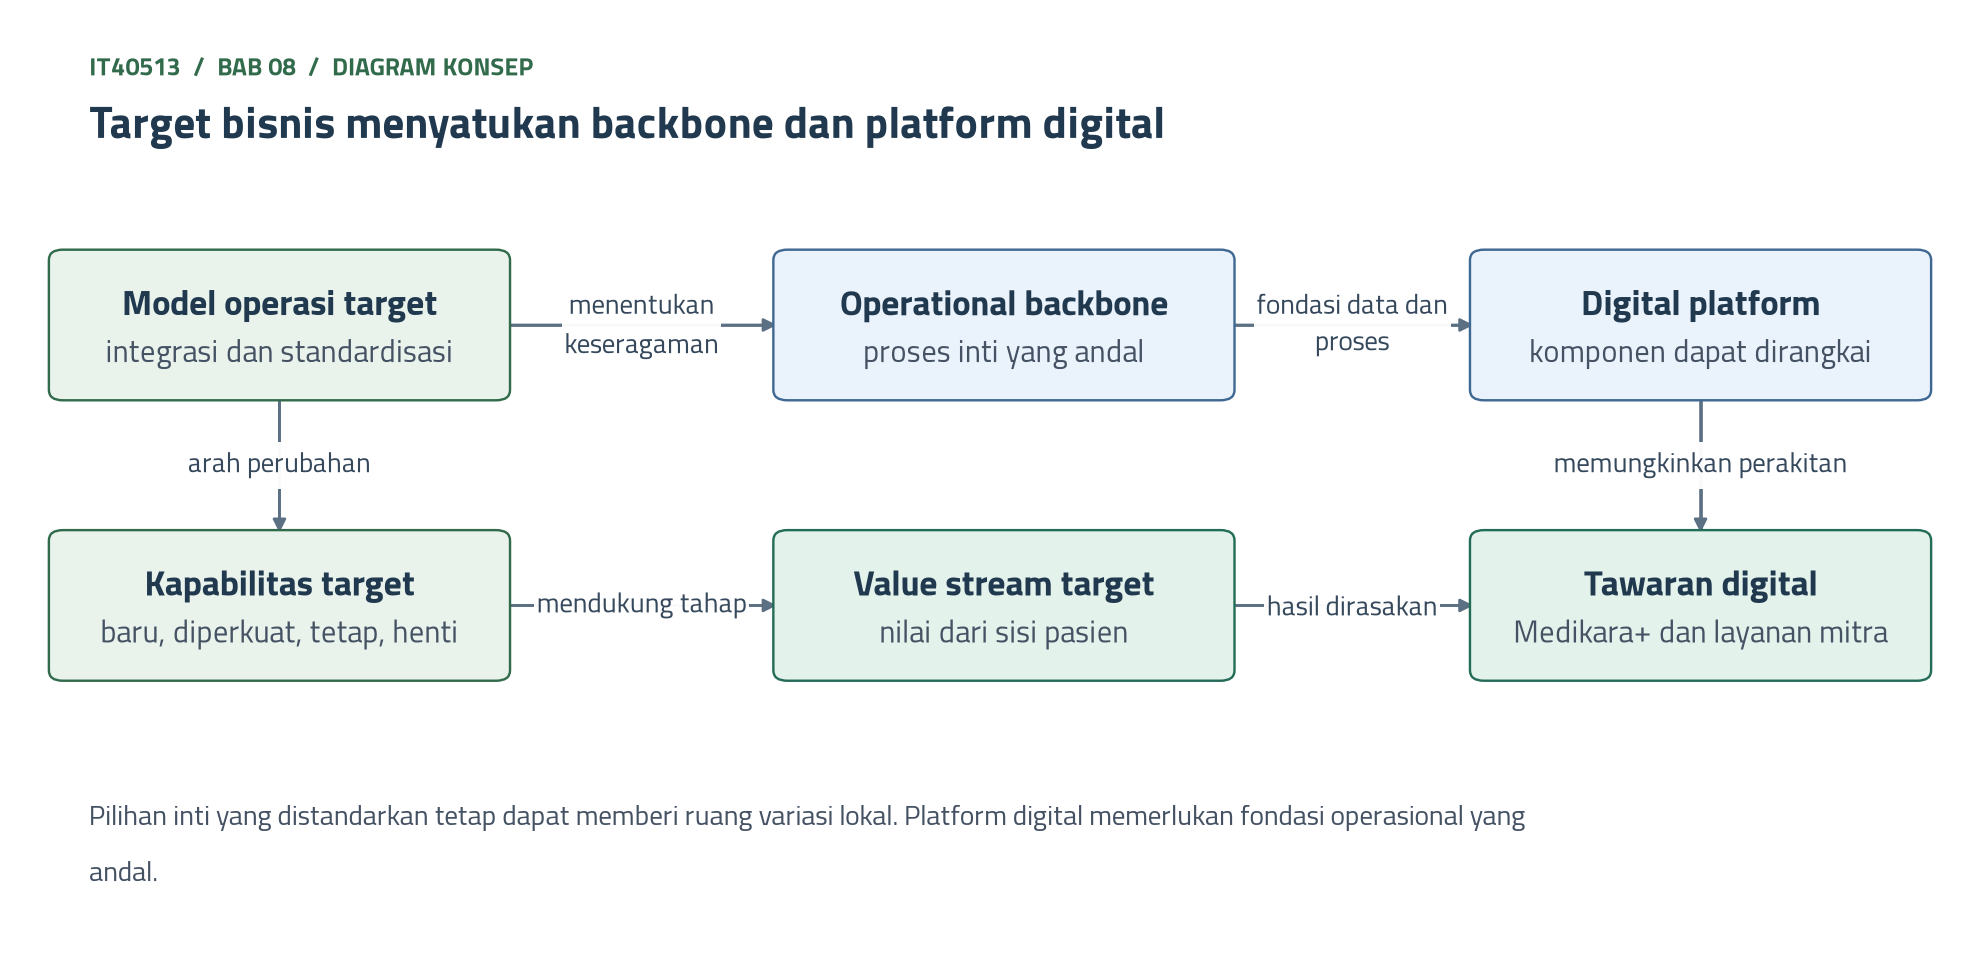
\includegraphics[width=0.96\textwidth,height=0.77\textheight,keepaspectratio]{../../figures/ch08-diagram-konsep.png}
  \label{fig:session08-ilustrasi-bab}
\end{frame}

\section{Transformasi Digital}

\begin{frame}{\hfill}
  \centering
  \Huge{\textbf{Transformasi Digital}}
\end{frame}

\begin{frame}{{\Large Tiga Fase Perubahan Digital}}
  \footnotesize
  \begin{tabularx}{\textwidth}{>{\raggedright\arraybackslash}p{2.3cm}
      >{\raggedright\arraybackslash}p{2.5cm} >{\raggedright\arraybackslash}p{2.9cm}
      >{\raggedright\arraybackslash}X}
    \hline
    \textbf{Fase} & \textbf{Yang berubah} & \textbf{Domain terdampak} &
      \textbf{Contoh Medikara} \\
    \hline
    Digitisasi & Media informasi & Data & Pemindaian berkas rekam medis lama \\
    \hline
    Digitalisasi & Proses yang sudah ada & Proses bisnis dan aplikasi & Pemesanan janji
      temu lewat Medikara+ \\
    \hline
    Trans\-for\-masi digital & Model bisnis & Seluruh domain, dimulai dari strategi & Paket
      kesehatan karyawan bersama mitra, dibayar bulanan \\
    \hline
  \end{tabularx}

  \vspace{8pt}
  \small Verhoef dan rekan-rekannya: sebagian besar literatur menganggap dua fase pertama perlu dilalui
  sebelum fase ketiga tercapai.
\end{frame}

\begin{frame}{{\Large Analogi dan Contoh Medikara}}
  \vspace{6pt}
  \small
  \begin{itemize}
    \item Analogi warung: memotret buku utang (digitisasi), menerima pesanan lewat pesan singkat
          (digitalisasi), menjadi titik ambil pesanan berkomisi (transformasi).
    \item Misalkan rumah sakit Bogor memindai sekitar 300.000 berkas dalam delapan bulan: digitisasi.
    \item Misalkan 28 persen kunjungan dipesan daring: digitalisasi.
    \item Transformasi: paket layanan kesehatan karyawan dengan pembayaran bulanan, bersama mitra.
    \item Program yang dianggarkan sebagai proyek aplikasi kehilangan bagian terpenting: perubahan model
          operasi, kapabilitas, dan tanggung jawab.
  \end{itemize}
\end{frame}

\begin{frame}{{\Large Lima Blok Designed for Digital}}
  \vspace{6pt}
  \small
  \begin{itemize}
    \item \textit{Shared customer insights}: pengetahuan bersama tentang kebutuhan pelanggan, diperoleh
          lewat percobaan yang diukur.
    \item \textit{Operational backbone}: sistem, data, dan proses terpadu yang mendukung operasi inti.
    \item \textit{Digital platform}: komponen bisnis, data, dan infrastruktur yang dapat dipakai ulang
          untuk merakit tawaran digital.
    \item \textit{Accountability framework}: pembagian tanggung jawab atas tawaran digital dan
          komponennya.
    \item \textit{External developer platform}: komponen digital yang dibuka bagi pihak luar.
  \end{itemize}
\end{frame}

\begin{frame}{{\Large Hubungan Kelima Blok}}
  \centering
  \eadiagram{../../figures/ch08-lima-blok.tex}
\end{frame}

\begin{frame}{{\Large Operational Backbone dan Digital Platform}}
  \scriptsize
  \begin{tabularx}{\textwidth}{l>{\raggedright\arraybackslash}X>{\raggedright\arraybackslash}X}
    \hline
    \textbf{Aspek} & \textbf{\textit{Operational backbone}} & \textbf{\textit{Digital platform}} \\
    \hline
    Pertanyaan & Apakah operasi inti berjalan andal dan efisien? &
      Seberapa cepat tawaran digital baru dapat dirakit? \\
    \hline
    Isi & Sistem transaksi, data induk, dan proses inti & Komponen yang dipakai ulang,
      misalnya jadwal, notifikasi, dan telekonsultasi \\
    \hline
    Ukuran & Ketepatan data, keandalan, biaya per transaksi & Waktu dari gagasan sampai
      peluncuran, tingkat pemakaian ulang komponen \\
    \hline
    Laju perubahan & Lambat dan terencana & Cepat dan sering, lewat percobaan \\
    \hline
    Contoh Medikara & SIMRS, ERP keuangan, identitas pasien tunggal, integrasi klaim BPJS
      Kesehatan & Komponen di balik Medikara+ yang dapat dipakai fitur lain dan mitra \\
    \hline
  \end{tabularx}

  \vspace{8pt}
  \small Urutannya tidak dapat dibalik: platform di atas data pasien yang kacau hanya menyebarkan
  kekacauan itu ke lebih banyak layar.
\end{frame}

\begin{frame}{{\Large Kasus: Medikara+ sebagai Calon Platform}}
  \begin{block}{Kasus Medikara Health}
    \small
    \begin{itemize}
      \item Medikara+ adalah tawaran digital. Platformnya adalah komponen di balik aplikasi itu.
      \item Identitas pasien di Medikara+ menjadi salinan keenam, di samping lima salinan SIMRS.
      \item Urutan target: rapikan \textit{operational backbone}, pisahkan \textit{digital platform},
            lalu buka sebagian komponen bagi mitra.
      \item Medikara+ belum punya pemilik tunggal: pemasaran membeli, TI memelihara, vendor mengubah.
      \item Data pemakaian aplikasi dan keluhan pasien belum pernah dianalisis bersama.
    \end{itemize}
  \end{block}
\end{frame}

\section{Model Operasi Target}

\begin{frame}{\hfill}
  \centering
  \Huge{\textbf{Model Operasi Target}}
\end{frame}

\begin{frame}{{\Large Pergeseran Model Operasi Medikara}}
  \centering
  {\small Integrasi: seberapa banyak data dipakai bersama. Standardisasi: seberapa seragam proses
  dijalankan.\par}
  \vspace{4pt}
  \eadiagram{../../figures/ch08-model-operasi.tex}
\end{frame}

\begin{frame}{{\Large Standardisasi dan Keleluasaan Lokal}}
  \scriptsize
  \begin{tabularx}{\textwidth}{>{\raggedright\arraybackslash}p{4.4cm}
      >{\raggedright\arraybackslash}p{2.5cm} >{\raggedright\arraybackslash}X}
    \hline
    \textbf{Bidang} & \textbf{Arah target} & \textbf{Alasan} \\
    \hline
    Identitas pasien dan pendaftaran & Distandarkan & Pasien dikenali sama di 5 rumah
      sakit, 18 klinik, laboratorium, dan 12 apotek \\
    \hline
    Isi minimum rekam medis & Distandarkan & Wajib terhubung ke platform interoperabilitas
      Kementerian Kesehatan \\
    \hline
    Kontrol akses data pasien & Distandarkan & Temuan audit internal dan insiden vendor 2025 \\
    \hline
    Klaim BPJS Kesehatan dan asuransi & Distandarkan & Aturan penjamin sama untuk semua
      fasilitas \\
    \hline
    Jadwal praktik dan layanan unggulan & Lokal & Kebutuhan pasien dan dokter tiap kota
      berbeda \\
    \hline
    Kemitraan setempat & Lokal, kontrak baku & Pasar berbeda, syarat berbagi data sama \\
    \hline
    Alur kerja perawatan di bangsal & Lokal, pedoman bersama & Budaya kerja dan susunan
      ruang tiap rumah sakit berbeda \\
    \hline
  \end{tabularx}
\end{frame}

\begin{frame}{{\Large Konsekuensi Model Operasi Target}}
  \vspace{6pt}
  \small
  \begin{itemize}
    \item Medikara kini berada di kuadran diversifikasi karena akuisisi, bukan karena dipilih.
    \item Strategi menuntut integrasi tinggi, sehingga target paling tidak berada di kuadran koordinasi.
    \item Struktur organisasi berubah: bidang yang distandarkan butuh pemilik lintas fasilitas, misalnya
          Kepala Layanan Pasien Terpadu.
    \item Data bersama bertambah: identitas pasien, isi rekam medis inti, dan data penjamin menjadi data
          perusahaan.
    \item Aplikasi bersama dibutuhkan. Pembagian ini menjadi masukan rasionalisasi aplikasi pada Bab 9.
  \end{itemize}
\end{frame}

\section{Opsi Kondisi Target}

\begin{frame}{\hfill}
  \centering
  \Huge{\textbf{Opsi Kondisi Target}}
\end{frame}

\begin{frame}{{\Large Dari Prinsip sampai Keputusan}}
  \centering
  \eadiagram{../../figures/ch08-alur-opsi.tex}

  \vspace{4pt}
  {\small Analogi: keluarga yang mencari rumah menyepakati kriteria lebih dahulu, baru melihat rumah.\par}
\end{frame}

\begin{frame}{{\Large Tiga Opsi Medikara}}
  \vspace{6pt}
  \small
  \begin{itemize}
    \item Opsi yang baik utuh, berbeda pada pilihan mendasar, dan bukan opsi boneka.
    \item Opsi A, sentralisasi penuh: pendaftaran, pusat kontak, dan penjadwalan dipusatkan di Jakarta.
          Satu SIMRS dalam 24 bulan. Posisinya unifikasi.
    \item Opsi B, inti yang distandarkan: identitas pasien, rekam medis inti, kontrol akses, dan klaim.
          Konsolidasi SIMRS bertahap sampai 2030. Posisinya koordinasi dengan inti yang seragam.
    \item Opsi C, federasi terintegrasi: kelima SIMRS dipertahankan, dibangun lapisan integrasi dan MPI
          (\textit{Master Patient Index}). Posisinya koordinasi dengan standardisasi paling rendah.
  \end{itemize}
\end{frame}

\begin{frame}{{\Large Matriks Kriteria Berbobot}}
  \footnotesize
  \begin{tabularx}{\textwidth}{>{\raggedright\arraybackslash}Xrrrr}
    \hline
    \textbf{Kriteria} & \textbf{Bobot} & \textbf{Opsi A} & \textbf{Opsi B} & \textbf{Opsi C} \\
    \hline
    Satu identitas dan satu rekam medis lintas fasilitas & 30\% & 5 (1,50) & 4 (1,20) &
      2 (0,60) \\
    \hline
    Pengalaman pasien: pendaftaran sekali, tunggu singkat & 20\% & 4 (0,80) & 4 (0,80) &
      2 (0,40) \\
    \hline
    Kepatuhan dan kontrol akses & 15\% & 5 (0,75) & 4 (0,60) & 3 (0,45) \\
    \hline
    Kelayakan dari kondisi saat ini & 20\% & 2 (0,40) & 4 (0,80) & 5 (1,00) \\
    \hline
    Biaya dan risiko perubahan & 15\% & 1 (0,15) & 3 (0,45) & 4 (0,60) \\
    \hline
    \textbf{Jumlah} & \textbf{100\%} & \textbf{3,60} & \textbf{3,85} & \textbf{3,05} \\
    \hline
  \end{tabularx}

  \vspace{6pt}
  \small Nilai 1 sampai 5, angka dalam kurung adalah nilai dikali bobot.
\end{frame}

\begin{frame}{{\Large Uji Kepekaan}}
  \footnotesize
  \begin{tabularx}{\textwidth}{>{\raggedright\arraybackslash}Xrrrl}
    \hline
    \textbf{Susunan bobot} & \textbf{Opsi A} & \textbf{Opsi B} & \textbf{Opsi C} &
      \textbf{Unggul} \\
    \hline
    Dasar: 30, 20, 15, 20, 15 & 3,60 & 3,85 & 3,05 & B \\
    \hline
    Integrasi dinaikkan, kelayakan diturunkan: 40, 20, 15, 10, 15 & 3,90 & 3,85 & 2,75 & A \\
    \hline
    Biaya dinaikkan, pengalaman diturunkan: 30, 10, 15, 20, 25 & 3,30 & 3,75 & 3,25 & B \\
    \hline
  \end{tabularx}

  \vspace{8pt}
  \small Opsi A hanya unggul bila bobot kelayakan dipangkas menjadi 10 persen. Pertanyaan yang diputuskan
  direksi: seberapa besar risiko pelaksanaan yang sanggup ditanggung organisasi.
\end{frame}

\begin{frame}{{\Large Business Scenario Medikara}}
  \scriptsize
  \begin{tabularx}{\textwidth}{>{\raggedright\arraybackslash}p{2.6cm}>{\raggedright\arraybackslash}X}
    \hline
    \textbf{Unsur} & \textbf{Isi: ``Pasien berpindah fasilitas''} \\
    \hline
    Masalah & Pasien yang berpindah fasilitas mendaftar ulang dan riwayatnya tidak terbaca
      dokter di fasilitas baru \\
    \hline
    Lingkungan & 5 rumah sakit dengan SIMRS berbeda versi, Medikara+ buatan vendor,
      integrasi \textit{point-to-point} ke BPJS Kesehatan dan SATUSEHAT \\
    \hline
    Tujuan SMART & Pada akhir 2028, 95 persen kunjungan rawat jalan di 5 rumah sakit
      dilayani dengan satu nomor pasien Medikara, dan riwayat lintas fasilitas terbuka bagi
      dokter yang merawat \\
    \hline
    Aktor & Manusia: pasien, petugas pendaftaran, dokter, apoteker, petugas klaim, klinik
      mitra. Komputer: Medikara+, lima SIMRS, MPI baru, sistem klaim, SATUSEHAT \\
    \hline
    Ukuran per aktor & Petugas memverifikasi pasien dalam 5 menit; dokter membuka riwayat
      lintas fasilitas tanpa meminta fotokopi \\
    \hline
    Alur kerja & Pasien klinik Depok dirujuk ke poli jantung di Jakarta, lalu kembali
      kontrol di Depok \\
    \hline
  \end{tabularx}

  \vspace{6pt}
  \small SMART: \textit{Specific, Measurable, Actionable, Realistic, Time-bound}.
\end{frame}

\begin{frame}{{\Large Kasus: Sentralisasi atau Inti Baku}}
  \begin{block}{Kasus Medikara Health}
    \small
    \begin{itemize}
      \item Direktur keuangan mendukung opsi A: biaya memelihara lima versi hilang.
      \item Direktur rumah sakit Bandung menolak. Misalkan dokter tamu berganti jadwal tiap minggu:
            perubahan hari yang sama dapat butuh dua hari.
      \item Alasan memilih opsi B: inti seragam, tanpa mengganti lima SIMRS sekaligus.
      \item Yang dikorbankan: penghematan pusat kontak tunggal tidak penuh, dan biaya pemeliharaan ganda
            berlanjut sampai 2030.
      \item Tinjau ulang: bila Juni 2028 kurang dari 80 persen pendaftaran memakai identitas terpadu.
    \end{itemize}
  \end{block}
\end{frame}

\section{Kapabilitas dan Value Stream}

\begin{frame}{\hfill}
  \centering
  \Huge{\textbf{Kapabilitas dan\\Value Stream}}
\end{frame}

\begin{frame}{{\Large Peta Kapabilitas Target}}
  \centering
  \eadiagram{../../figures/ch08-peta-kapabilitas.tex}

  \vspace{4pt}
  {\small 18 kapabilitas tingkat 2: 3 baru, 8 diperkuat, 5 dipertahankan, dan 2 dihentikan.\par}
\end{frame}

\begin{frame}{{\Large Perubahan Kapabilitas Medikara}}
  \scriptsize
  \begin{tabularx}{\textwidth}{>{\raggedright\arraybackslash}p{5.6cm}lc>{\raggedright\arraybackslash}X}
    \hline
    \textbf{Kapabilitas} & \textbf{Jenis} & \textbf{Tingkat} & \textbf{Pemicu} \\
    \hline
    Pengelolaan Identitas Pasien Terpadu & baru & -- ke 3 & Strategi satu rekam medis \\
    \hline
    Pengelolaan Kemitraan Ekosistem & baru & -- ke 2 & Strategi ekosistem mitra \\
    \hline
    Wawasan Pasien dan Analitik & baru & -- ke 2 & Data Medikara+ belum dianalisis \\
    \hline
    Pengelolaan Kepatuhan & diperkuat & 2 ke 3 & Data pribadi, rekam medis \\
    \hline
    Pendaftaran Pasien & diperkuat & 2 ke 3 & Pendaftaran masih per fasilitas \\
    \hline
    Penjadwalan Layanan & diperkuat & 2 ke 3 & Antrean yang panjang \\
    \hline
    Pengelolaan Rekam Medis & diperkuat & 1 ke 3 & Data pasien tersebar \\
    \hline
    Telekonsultasi & diperkuat & 2 ke 3 & Komponen terkunci di vendor \\
    \hline
    Klaim dan Penjaminan & diperkuat & 2 ke 3 & Biaya integrasi tinggi \\
    \hline
    Pengelolaan Akses Pengguna & diperkuat & 1 ke 3 & Temuan audit kontrol akses \\
    \hline
    Pelaporan Manajemen & diperkuat & 1 ke 3 & Laporan dari \textit{spreadsheet} \\
    \hline
    Penerbitan Nomor Rekam Medis Lokal & dihentikan & 2 ke -- & Diganti identitas terpadu \\
    \hline
    Rekonsiliasi Data Manual Antarfasilitas & dihentikan & 1 ke -- & Data dipakai bersama \\
    \hline
  \end{tabularx}
\end{frame}

\begin{frame}{{\Large Menghentikan dan Menambah Kapabilitas}}
  \vspace{6pt}
  \small
  \begin{itemize}
    \item Menghentikan kapabilitas berarti menghentikan pekerjaan orang, sehingga butuh rencana
          pengalihan tugas.
    \item Nomor rekam medis lokal tercetak di label sampel, gelang pasien, dan arsip kertas. Tabel padanan
          tetap dipelihara bertahun-tahun.
    \item Pengelolaan Kemitraan Ekosistem muncul karena strategi 2026 sampai 2030.
    \item Mitra merujuk pasien yang sama, sehingga identitas terpadu berjalan lebih dahulu.
    \item Misalkan target 40 klinik mitra, tiga bulan per klinik. Satu tim yang mengerjakannya berurutan
          butuh sepuluh tahun.
  \end{itemize}
\end{frame}

\begin{frame}{{\Large Value Stream Target Rawat Jalan}}
  \centering
  \eadiagram{../../figures/ch08-value-stream-target.tex}
\end{frame}

\begin{frame}{{\Large Ukuran Keberhasilan Tiap Tahap}}
  \scriptsize
  \begin{tabularx}{\textwidth}{>{\raggedright\arraybackslash}p{3.3cm}>{\raggedright\arraybackslash}Xrr>{\raggedright\arraybackslash}p{3.2cm}}
    \hline
    \textbf{Tahap} & \textbf{Ukuran} & \textbf{Kini} & \textbf{2030} & \textbf{Kapabilitas} \\
    \hline
    1. Memesan layanan & Janji temu dipesan daring & 28\% & 50\% & Penjadwalan Layanan \\
    \hline
    2. Hadir dan terverifikasi & Median menit dari datang sampai terverifikasi & 25 & 5 &
      Pengelolaan Identitas Pasien Terpadu \\
    \hline
    3. Diperiksa dan didiagnosis & Riwayat lintas fasilitas terbuka & 10\% & 95\% &
      Pengelolaan Rekam Medis \\
    \hline
    4. Menerima obat & Median menit menunggu obat nonracikan & 45 & 20 & Layanan Farmasi
      dan Laboratorium \\
    \hline
    5. Menyelesaikan pembayaran & Klaim BPJS dikembalikan & 9\% & 3\% & Klaim dan
      Penjaminan \\
    \hline
    6. Ditindaklanjuti & Pasien kontrol menerima pengingat & 20\% & 90\% & Telekonsultasi \\
    \hline
  \end{tabularx}

  \vspace{6pt}
  \small Tiga waktu tunggu terbesar: kini $25 + 70 + 45 = 140$ menit. Misalkan tunggu dokter menjadi 30
  menit, jumlah target $5 + 30 + 20 = 55$ menit.
\end{frame}

\begin{frame}{{\Large Kasus: Satu Identitas Lintas Fasilitas}}
  \begin{block}{Kasus Medikara Health}
    \small
    \begin{itemize}
      \item Misalkan pasien diabetes klinik pratama Depok dirujuk ke poli jantung di Jakarta.
      \item Kini: mendaftar ulang, nomor rekam medis baru, membawa fotokopi hasil laboratorium, dan dokter
            jantung tidak melihat daftar obat dari klinik.
      \item Target: dikenali dengan nomor pasien Medikara yang sama. Dokter membuka riwayat dari klinik
            Depok, dan resep elektronik dikirim ke apotek terdekat.
      \item Perubahan ini tidak membutuhkan dokter yang bekerja lebih cepat.
      \item Tahap 2, 3, dan 4 bersandar pada identitas yang dikenali di seluruh jaringan.
    \end{itemize}
  \end{block}
\end{frame}

\section{Aktivitas dan Latihan}

\begin{frame}{\hfill}
  \centering
  \Huge{\textbf{Aktivitas dan Latihan}}
\end{frame}

\begin{frame}{{\Large Aktivitas: Memilih Opsi Kondisi Target}}
  \scriptsize
  \begin{tabularx}{\textwidth}{l>{\raggedright\arraybackslash}X>{\raggedright\arraybackslash}p{3.4cm}}
    \hline
    \textbf{Peran} & \textbf{Tugas utama} & \textbf{Yang diserahkan} \\
    \hline
    Analis bisnis & Memimpin perumusan opsi dan kriteria, memastikan kriteria diturunkan
      dari prinsip C1 & Uraian opsi dan bobot kriteria \\
    \hline
    Analis teknologi & Menilai kelayakan tiap opsi dari kondisi saat ini (C2), terutama
      aplikasi dan integrasi & Nilai kelayakan beserta alasannya \\
    \hline
    Pemodel & Menandai perubahan kapabilitas pada \textit{capability map} dan memperbarui
      model di Archi & Peta kapabilitas target \\
    \hline
    Koordinator & Memandu penilaian, menulis catatan keputusan, dan menyelaraskan dengan
      tiga mata kuliah lain & Catatan keputusan \\
    \hline
  \end{tabularx}

  \vspace{4pt}
  \small
  \begin{itemize}
    \item Susun dua sampai tiga opsi, lalu sepakati bobot sebelum opsi dinilai.
    \item Uji kepekaan: ubah bobot dua kriteria terbesar sebesar 10 poin.
    \item Pilih satu opsi, tandai kapabilitas, dan rancang \textit{value stream} target.
  \end{itemize}
\end{frame}

\begin{frame}{{\Large Luaran C3 dan Kriteria Penilaian}}
  \footnotesize
  \begin{tabularx}{\textwidth}{>{\raggedright\arraybackslash}Xr}
    \hline
    \textbf{Kriteria} & \textbf{Bobot} \\
    \hline
    Opsi berbeda pada pilihan mendasar, tanpa opsi boneka & 20\% \\
    \hline
    Kriteria diturunkan dari prinsip C1, dan bobot disepakati sebelum penilaian & 20\% \\
    \hline
    Alasan, hal yang dikorbankan, dan hasil uji kepekaan tertulis jelas & 25\% \\
    \hline
    Peta kapabilitas dan \textit{value stream} konsisten dengan opsi terpilih & 20\% \\
    \hline
    Ukuran keberhasilan terukur, dengan angka saat ini dan target & 15\% \\
    \hline
  \end{tabularx}

  \vspace{8pt}
  \small Luaran: model operasi target, matriks opsi dan catatan keputusan, \textit{capability map} target,
  dan \textit{value stream} target. Berkas pendukung: \berkas{sources/chapter08/README.md}.
\end{frame}

\begin{frame}{{\Large Ringkasan}}
  \vspace{6pt}
  \small
  \begin{itemize}
    \item Digitisasi memindahkan media, digitalisasi mengubah proses, transformasi digital mengubah cara
          menciptakan dan menangkap nilai.
    \item \textit{Operational backbone} lebih dahulu, baru \textit{digital platform}.
    \item Medikara bergeser dari diversifikasi menuju koordinasi dengan inti yang seragam.
    \item Opsi inti yang distandarkan unggul dengan 3,85. Tiga waktu tunggu terbesar ditargetkan turun
          dari 140 menjadi 55 menit.
    \item Pesan utama: arsitektur bisnis target bukan daftar sistem yang akan dibeli, melainkan keputusan
          tentang apa yang diseragamkan, apa yang dikorbankan, dan bagaimana keberhasilannya diukur.
  \end{itemize}
\end{frame}

\begin{frame}{{\Large Latihan}}
  \vspace{6pt}
  \small
  \begin{enumerate}
    \item Membedakan Operational Backbone dan Digital Platform: golongkan enam sampai delapan komponen
          menurut pertanyaan yang dijawab tiap komponen.
    \item Menulis \textit{Tradeoff} Sentralisasi untuk Direksi: tulis yang diperoleh dan yang dikorbankan
          untuk tiga sampai empat aspek, lalu ringkas menjadi tepat tiga kalimat.
    \item Syarat Kapabilitas Pengelolaan Kemitraan: jelaskan mengapa kapabilitas ini tidak tampak pada
          \textit{capability map} saat ini, lalu daftar tiga sampai lima syarat agar berjalan.
  \end{enumerate}
\end{frame}

\begin{frame}{{\Large Bacaan dan Berkas Pendukung}}
  \vspace{10pt}
  \begin{itemize}
    \item \href{https://doi.org/10.1016/j.jbusres.2019.09.022}{\textit{Digital Transformation: A Multidisciplinary Reflection and Research Agenda}}
    \item \href{https://www.opengroup.org/togaf}{\textit{The TOGAF Standard, 10th Edition (2025 Update)}}
    \item \href{https://publications.opengroup.org/g176}{\textit{TOGAF Series Guide: Business Scenarios}}
    \item \berkas{sources/chapter08/README.md}
  \end{itemize}
\end{frame}

\end{document}
